\documentclass{article}
	
\usepackage[margin=1in]{geometry}		% For setting margins
\usepackage{amsmath}				% For Math
\usepackage[]{amssymb}
\usepackage{amsmath}
\usepackage{gensymb}
\usepackage{fancyhdr}				% For fancy header/footer
\usepackage{graphicx}				% For including figure/image
\usepackage{cancel}					% To use the slash to cancel out stuff in work
\usepackage{wasysym}                % For cent symbol
\usepackage{needspace}              % To force item to next page
\usepackage{mathtools}

%%%%%%%%%%%%%%%%%%%%%%
% Set up fancy header/footer
\pagestyle{fancy}
\fancyhead[RO,R]{{\large\textbf{PHYS-102}}}
\fancyhead[LO,L]{\large{\textbf{Ch 33 Problem Set}}}
% \fancyhead[CO,C]{\large{\textbf{Part 1}}}
% \fancyhead[RO,R]{\today}
\fancyfoot[LO,L]{}
\fancyfoot[CO,C]{\thepage}
\fancyfoot[RO,R]{}
\renewcommand{\headrulewidth}{0.4pt}
\renewcommand{\footrulewidth}{0.4pt}
%%%%%%%%%%%%%%%%%%%%%%

\newcommand{\hmwkTitle}{Chapter 33 Lenses and Optical Instruments}
% \newcommand{\hmwkDueDate}{February 12, 2014}
\newcommand{\hmwkClass}{PHYS-102}
% \newcommand{\hmwkClassTime}{}
% \newcommand{\hmwkClassInstructor}{Professor Isaac Newton}
\newcommand{\hmwkAuthorName}{\textbf{\underline{\hspace{3in}}}}

% math shortcuts
\newcommand\rr{\quad\Rightarrow\quad}
\newcommand{\spc}{\vspace{1em}\hrule\vspace{1em}}
\newcommand{\bp}[1]{\left(#1\right)}
\newcommand{\bb}[1]{\left[#1\right]}

%
% Title Page
%

\title{
    \vspace{2in}
    \textmd{\textbf{\hmwkTitle}}\\
    \vspace{0.5in}
    \textmd{\textbf{\hmwkClass}}\\
    % \normalsize\vspace{0.1in}\small{Due\ on\ \hmwkDueDate\ at 3:10pm}\\
    % \vspace{0.1in}\large{\textit{\hmwkClassInstructor\ \hmwkClassTime}}
    \vspace{4in}
}

\author{\hmwkAuthorName}
\date{}
\begin{document}
\maketitle
\newpage
\begin{center}
    \section*{\textbf{\underline {Conceptual Questions}}}
\end{center}
\subsubsection*{
    1. Where must the film be placed if a camera lens is to make a sharp image
    of an object far away?
}
\subsubsection*{
    3.  Can a diverging lens form a real image under any circumstances? Explain. 
}
\subsubsection*{
    8. Compare the mirror equation with the thin lens equation. Discuss similarities
    and differences, especially the sign conventions for the quantities involved.
}
\subsubsection*{
    14. The thicker a double convex lens is in the center as compared to its edges,
    the shorter its focal length for a given lens diameter. Explain.
}
\subsubsection*{
    19. You can tell whether people are nearsighted or farsighted by looking at the
    width of their fa e through their glasses. If a person’s face appears narrower
    through the glasses, is the person farsighted or nearsighted? 
}
\begin{figure}[h]
    \begin{center}
        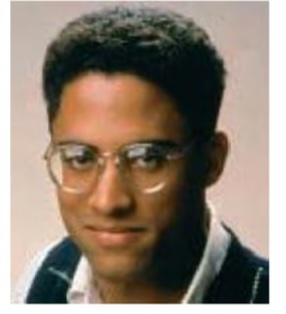
\includegraphics[width=0.3\textwidth]{figures/q19.jpg}
    \end{center}
\end{figure}
\subsubsection*{
    20. The human eye is much like a camera - yet, when a camera shutter is left open
    and the camera is moved, the image will be blurred. But when you move your head
    with your eyes open, you still see clearly. Explain.
}
\subsubsection*{
    26. For both converging and diverging lenses discuss how the focal length
        from red light differs from that for violet light 
}
\newpage
\begin{center}
    \section*{\textbf{\underline {Problems}}}
    \subsection*{\textbf{\textit{Placeholder}}}
\end{center}
\subsubsection*{
    1. 
}
\subsubsection*{
    2. 
}
\subsubsection*{
    4. 
}
\subsubsection*{
    6. 
}
\subsubsection*{
    10. 
}
\subsubsection*{
    12. 
}
\subsubsection*{
    13. 
}
\subsubsection*{
    14. 
}
\subsubsection*{
    20. 
}
\subsubsection*{
    21. 
}
\subsubsection*{
    26. 
}
\subsubsection*{
    27. 
}
\subsubsection*{
    28. 
}
\subsubsection*{
    29. 
}
\subsubsection*{
    33. 
}
\subsubsection*{
    41. 
}
\subsubsection*{
    42. 
}
\subsubsection*{
    45. 
}
\subsubsection*{
    46. 
}
\subsubsection*{
    48. 
}
\subsubsection*{
    60. 
}
\subsubsection*{
    63. 
}
\subsubsection*{
    87. 
}
\end{document}
